\section{Two stage optimization}
\label{sec:twoStage}
To solve the Mode Selection problem (Section \ref{sec:mode selection}), we propose a two stage solution. 
The first stage is offline (Fig. \ref{fig:juicyj} left): in it, we thoroughly profile the perception algorithm's throughput $T(\sigma,F_c,F_g)$ and power consumption $P(\sigma,F_c,F_g)$ for various values of the hardware knobs $\sigma$, $F_c$ and $F_g$. 
The second stage is at runtime (Fig. \ref{fig:juicyj} right): based on the current control error, a supervisor chooses a weighting of throughput and power; intuitively, the larger the error, the more weight throughput receives, and vice-versa.
The supervisor then picks the task schedule $\sigma$ and CPU-GPU frequencies $F_c,F_g$ that best maximize the weighted combination of throughput and power.
A high-level view of this approach is shown in Fig. \ref{fig:juicyj}. 
We next detail each stage.

\subsection{Offline profiling of performance and power consumption of the perception algorithm}
\label{sec:profiling}
\begin{figure}
	\centering
	\includegraphics[scale=0.3]{Figs/vanishing}
	\caption{The vanishing point algorithm with components running on either CPU or GPU at various frequencies, resulting in different power consumptions and execution times.}
	\label{fig:vanishing}		
\end{figure}

For the perception algorithm, the first stage of our method is profiling the performance (timing and, if available, quality) and power consumption of the computation. With the vanishing point algorithm, we can execute the Blur, the Edge detection and the Hough transform on either the CPU or the GPU (Fig. \ref{fig:vanishing}. RANSAC runs fast enough to not have a significant impact on the total execution time, so we do not consider running it on the GPU. Execution on the GPU results, in general, in a speed-up over the CPU but at the cost of higher power draw from the Jetson. Additionally, on the Jetson, we can control the performance of the CPU and GPU by changing the clock frequencies at which they operate. This gives us multi-dimensional knobs on the hardware level that we can control to trade-off computation speed and power consumption.

To do this profiling offline, we first navigate the robot manually in corridors and log video from the on-board camera at a high frame-rate (60Hz). 
We run Vanishing point algorithm on this video offline and profile it with different scheduling of the three components (Blur, Canny and Hough) on the CPU and GPU, and at different frequencies of both processors.

We wrote a custom C-code library to log power measurements from a Tektronix PWS4205 Programmable DC power supply at 100Hz. 
For this we communicate with the power supply over USB using the USB Test and Measurement Class (USB-TMC) communication protocol. 
 
Since for an algorithm like Vanishing point there is no well-defined notion of ground truth, we do not have a measure of accuracy of the algorithm. 
Instead, Vanishing point's update rate (which is the inverse of the computation time) is used as a performance measure, since with faster updates the controller has less delay, resulting in better control performance. 

\subsubsection{Experimental results for profiling}
%profilingresults


Figure \ref{fig:dfsa} shows the profiling results for the throughput (update rate) of the Vanishing Point algorithm for different CPU-GPU allocations of the 3 tasks and different frequencies of the CPU and the GPU. 
Note, the CPU can be clocked upto 2.32 GHz (on all 4 cores), while the GPU can be clocked upto 0.852 GHz. 
We select 6 operating frequencies evenly spaced from the minimum and maximum Jetson CPU and GPU frequencies for both the CPU and the GPU. 
In these figures, the 3 letter combinations encode the CPU-GPU allocation .
For example, C G C means that the Blur was run on the CPU, Canny on the GPU and the Hough transform on the CPU.


\begin{figure}[htbp]
	\centering
	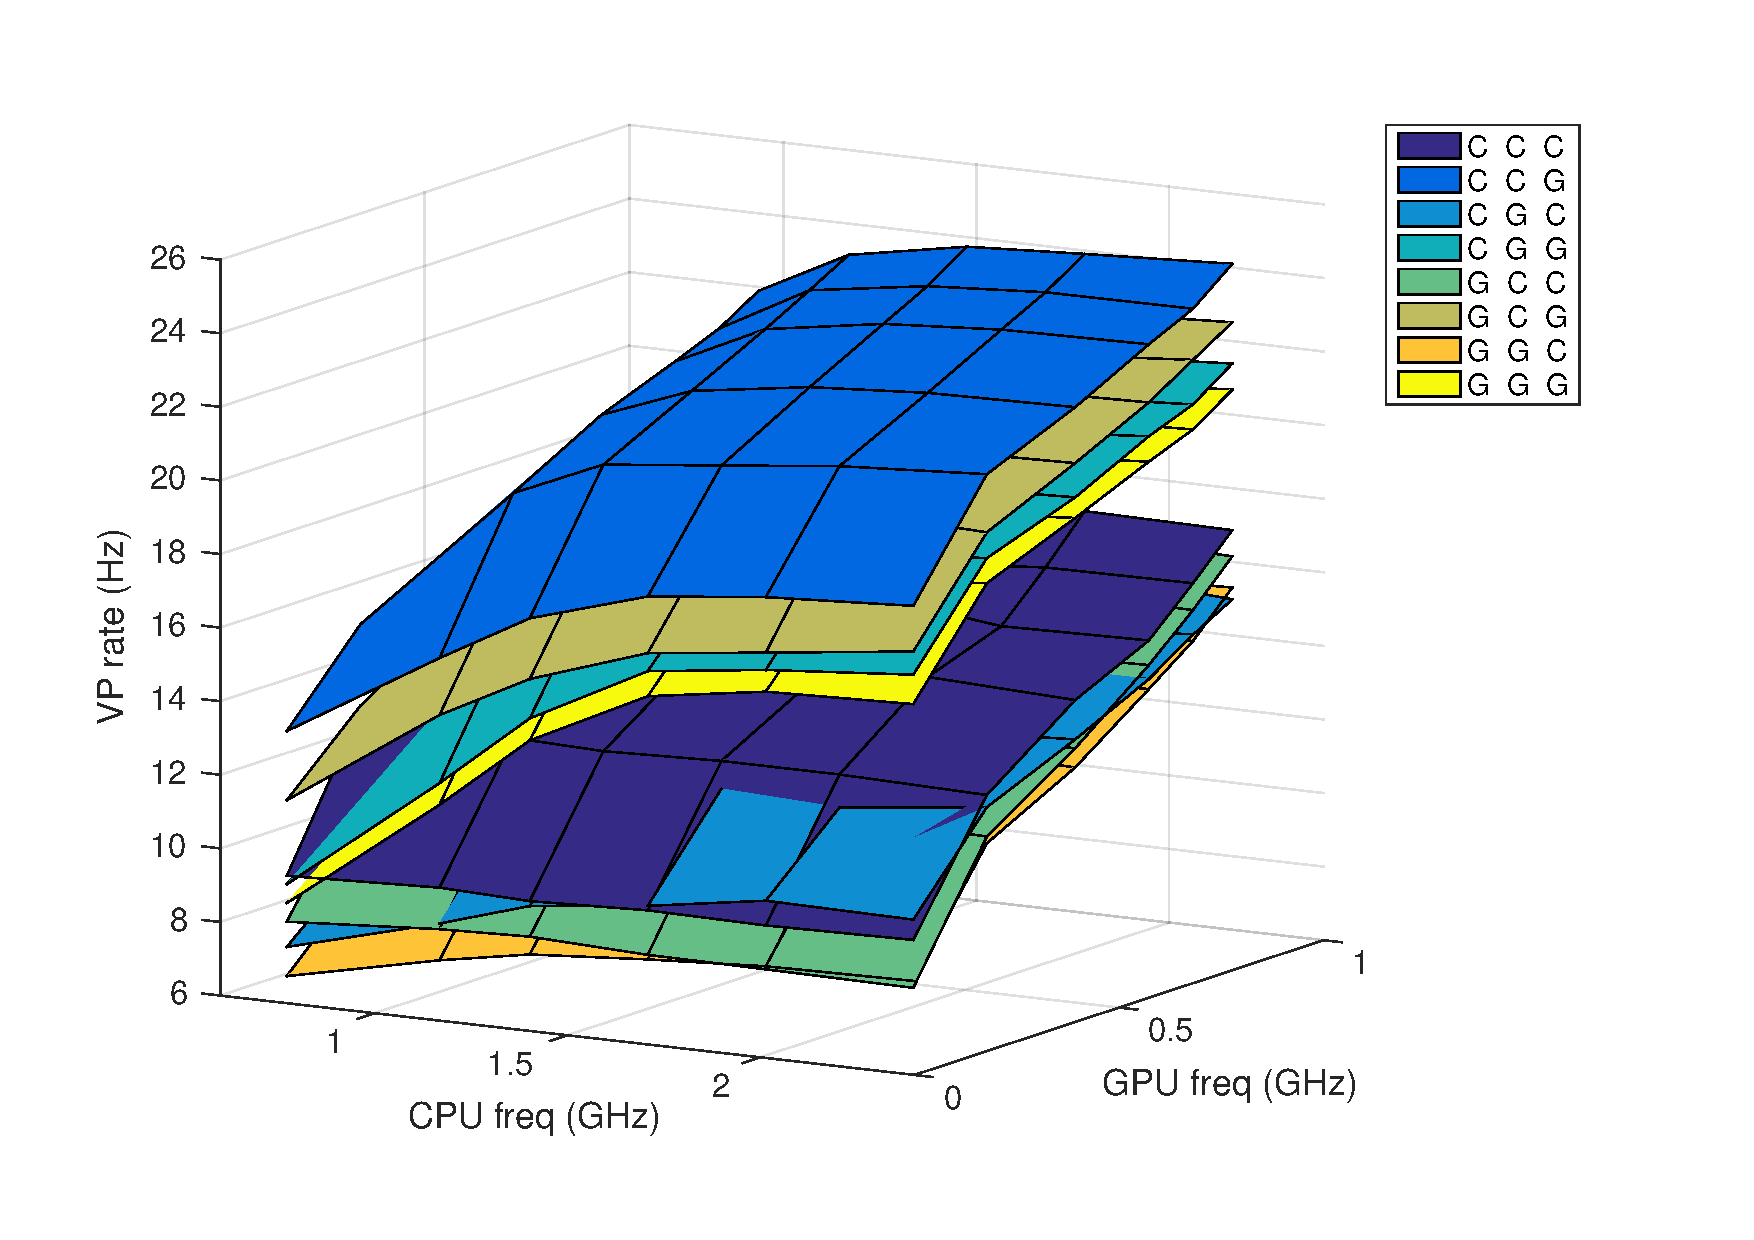
\includegraphics[width=0.46\textwidth]{Figs/surf_Rate.pdf}
	\caption{Vanishing point algorithm update rate for different CPU-GPU assignments at varying frequencies (color in online version).}
	\label{fig:sfda}%same freq diff assignment}
\end{figure}

%\begin{figure}[hbtp]
%\centering
%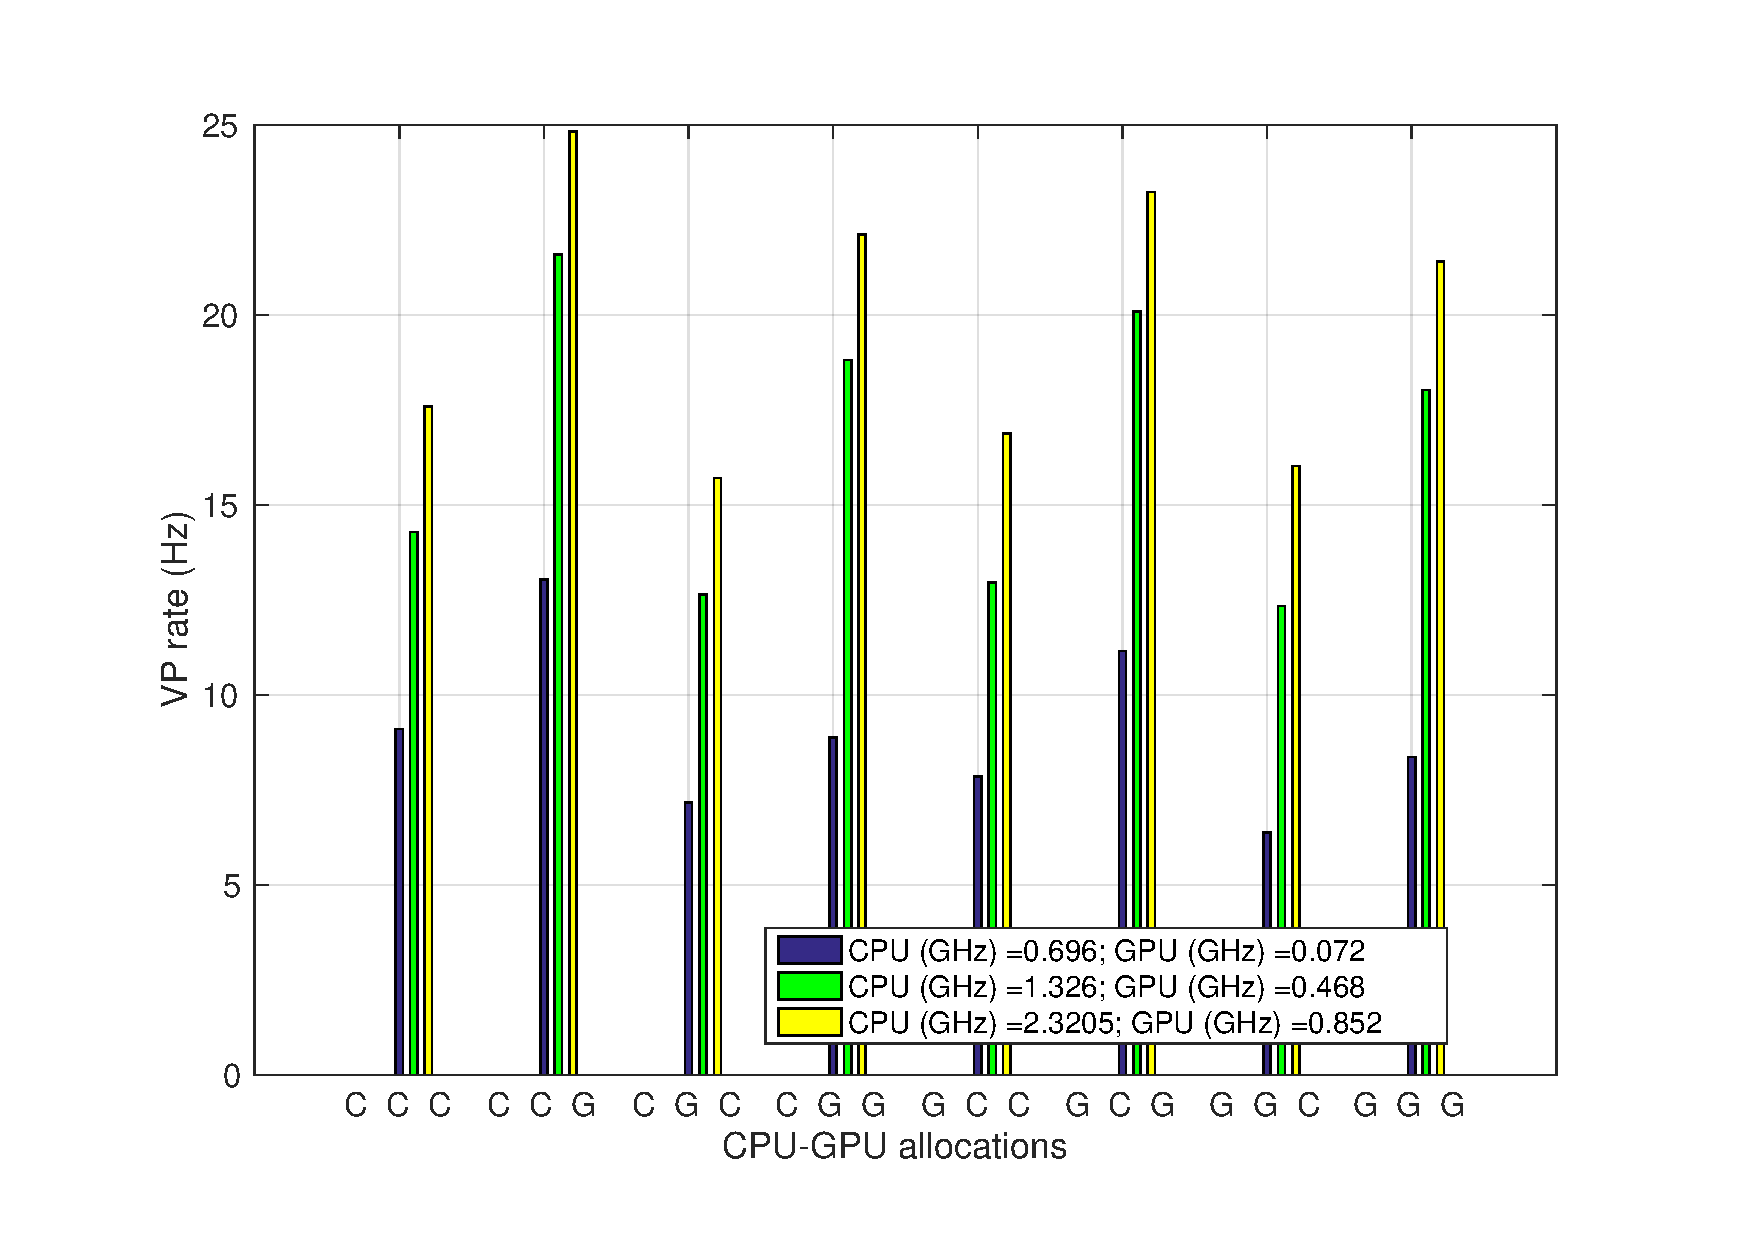
\includegraphics[scale=0.3]{Figs/RateHist.pdf}
%\caption{Control update rate for different frequencies and a given CPU-GPU assignment. For clarity we only consider 3 CPU and GPU frequencies for this %figure, ranging from the minimum to the maximum of frequencies of CPU and GPU. (Color in online version) }
%\label{fig:dfsa} %diff freq same assignment}
%\end{figure}

Figure \ref{fig:sfda_pow} showS the profiling of average power consumed during the computations for the vanishing point over all frames in the video used for the profiling.


\begin{figure}[htbp]
	\centering
	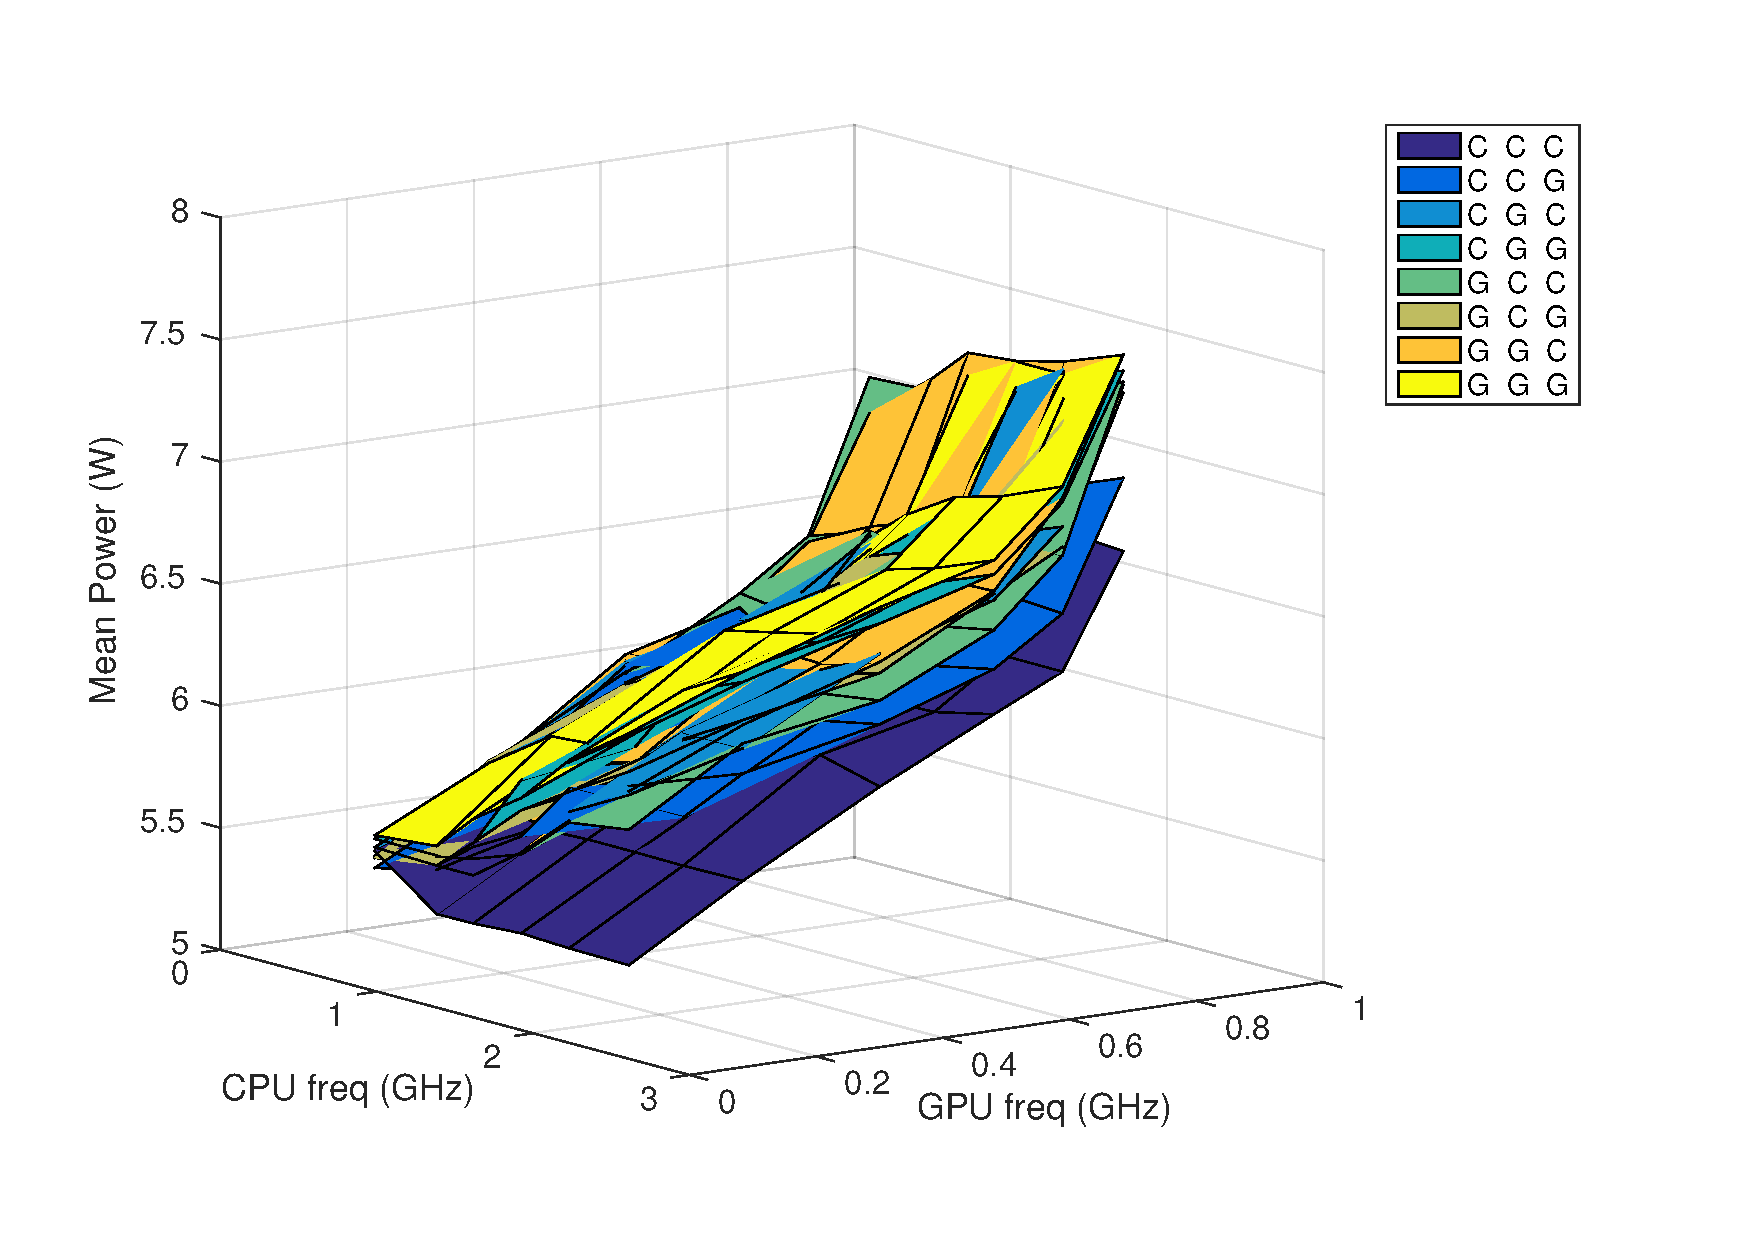
\includegraphics[width=0.46\textwidth]{Figs/surf_Power.pdf}
	\caption{Mean power consumed by the Jetson for different CPU-GPU assignments at varying frequencies. (Color in online version)}
	\label{fig:sfda_pow}%same freq diff assignment}
\end{figure}

%\begin{figure}[htbp]
%\centering
%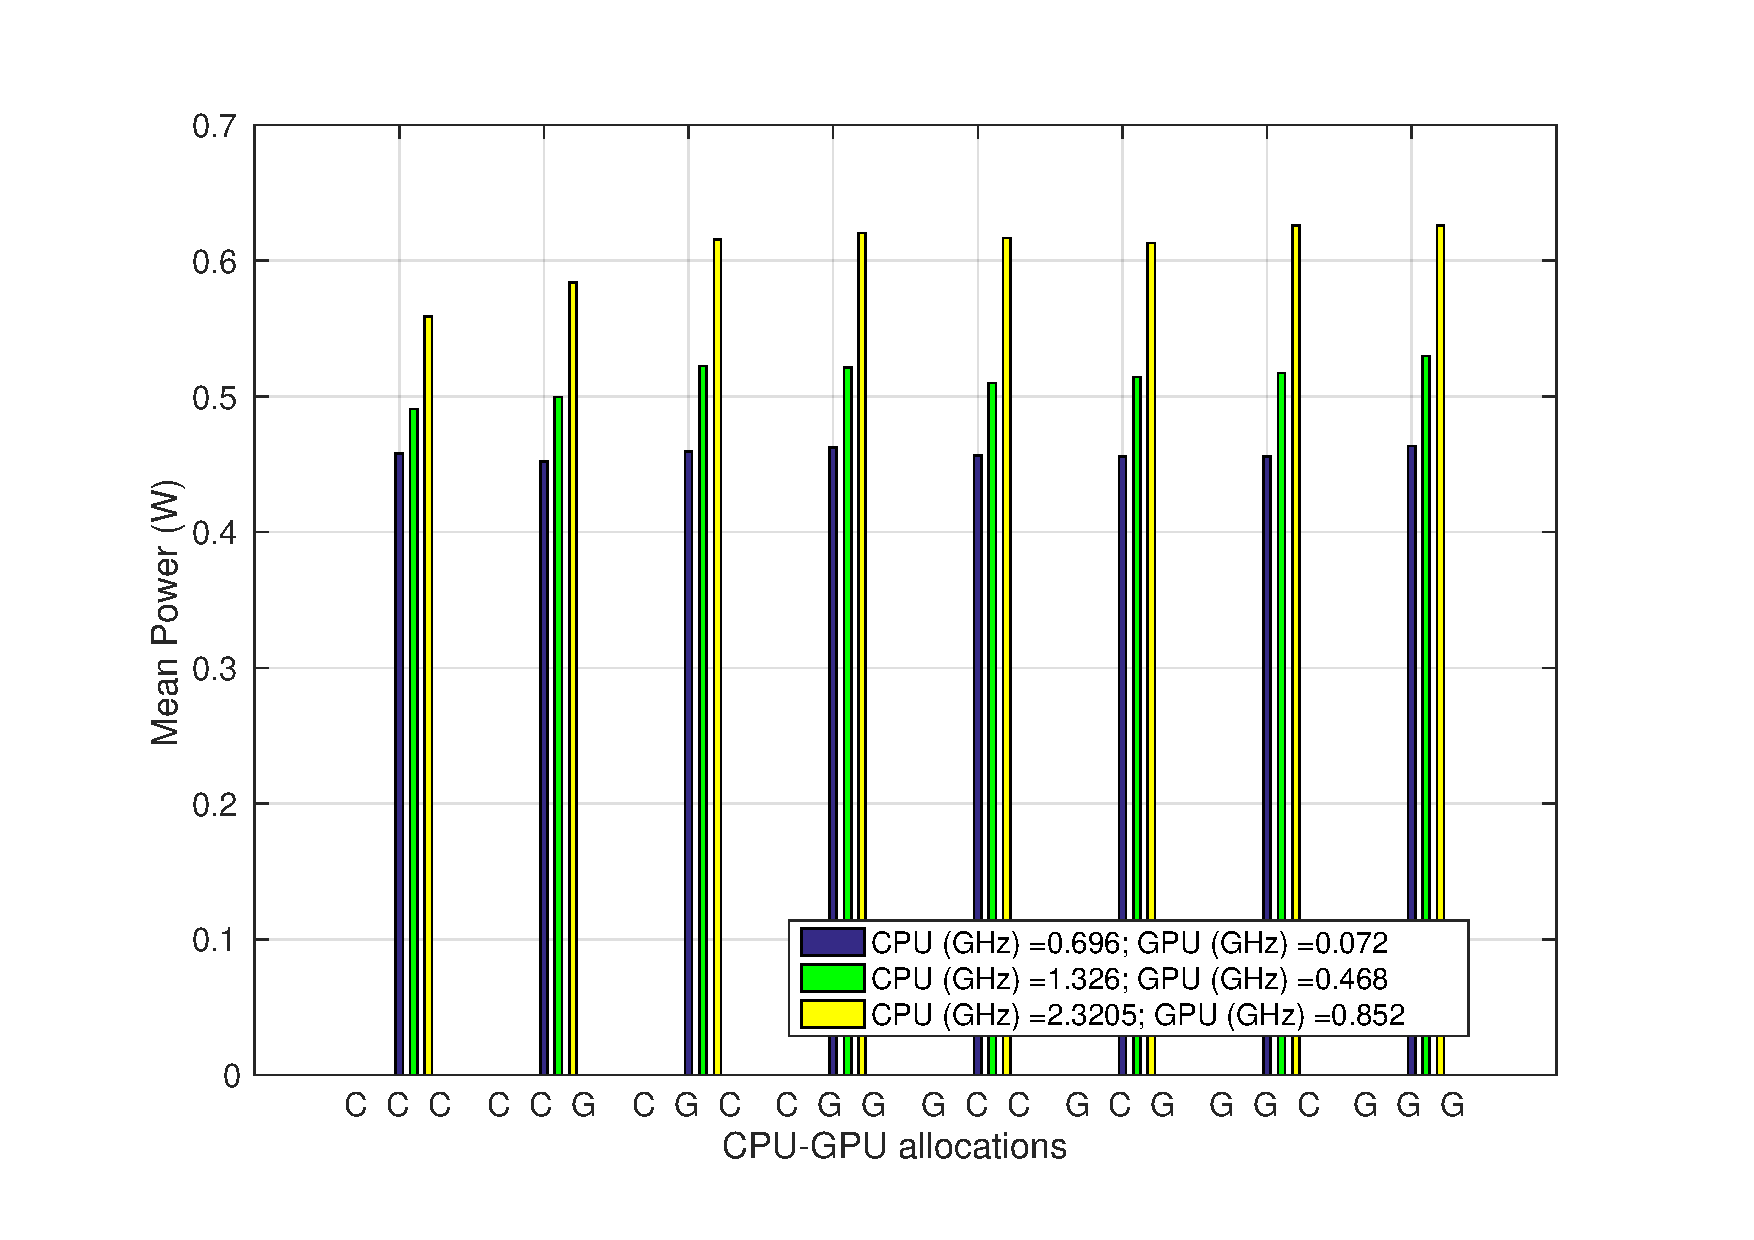
\includegraphics[width=0.46\textwidth]{Figs/PowerHist.pdf}
%\caption{Mean power consumed by the Jetson for different frequencies and a given CPU-GPU assignment.  For clarity we only consider 3 CPU and GPU frequencies for this figure, ranging from the minimum and maximum of both the CPU and the GPU. (Color in online version)}
%\label{fig:dfsa_pow} %diff freq same assignment}
%\end{figure}


\subsection{Feedback driven online scheduling and mode selection}
\label{sec:scheduling}

The profiling results indicate that the knobs $\sigma, F_c$ and $F_g$ allow us to trade-off throughput for power, as expected.
At runtime, we must decide which knob setting to choose at every time step. 
This is done by maximizing the following objective function at every time step $t$:

\begin{equation}
\max_{\sigma,F_{c},F_{g}} \alpha(x_m,x_v)\mathbf{\bar{T}}(\sigma,F_{c},F_{g}) + \frac{1-\alpha(x_m,x_v)}{\mathbf{E[\bar{P}]}(\sigma,F_{c},F_{g})}
\label{eq:cost_runtime}
\end{equation}

Recall that $\mathbf{\bar{T}}(\sigma,F_{c},F_{g})$ is the normalized throughput of VP, and $\mathbf{E[\bar{P}]}(\sigma,F_{c},F_{g})$ is the mean normalized power consumed by the computation platform.
The parameter $\alpha(x_m,x_v) \in [0,1]$ determines how much to weigh throughput versus performance at every time step. 
It is computed as a function of the abscissa $x_m,x_v$: recall that non-zero values of either indicates deviation from the center line of the corridor (Section \ref{sec:vp}). 
Since $x_m,x_v$ are time-varying, $\alpha$ is also time-varying.
As $x_m$ or $x_v$ deviates further away from 0, $\alpha$ increases to more heavily weigh throughput, thus skewing the optimization towards larger throughput and better control performance.
This translates as different CPU-GPU schedules and different frequencies.
In this paper, we use three different functions for $\alpha$, given $d >0$:

{\footnotesize{
		\begin{equation}
		\alpha= f_1(x_v(t)) = \\
		\begin{cases}
		0.001,&\text{if }x_v(t)\in[-d,d]\\
		x_v(t)+d,&\text{if }x_v(t)<-d\\
		x_v(t)-d,&\text{if }x_v(t)>d
		\end{cases}
		\label{eq:f1}
		\end{equation}
	}}
	
	{\footnotesize{
			\begin{equation}
			\alpha = f_2(x_m(t)) = \\
			\begin{cases}
			0.001,&\text{if }x_m(t)\in[-d,d]\\
			x_m(t)+d,&\text{if }x_m(t)<-d\\
			x_m(t)-d,&\text{if }x_m(t)>d
			\end{cases}
			\label{eq:f2}
			\end{equation}
		}}
		
{\footnotesize{
		\begin{equation}
		\alpha = f_3(x_m(t),x_v(t)) \\
		\begin{cases}
		0.001,\text{if }|x_m(t)|+|x_v(t)|<d\\
		|x_m(t)|+|x_v(t)|-d,\text{otherwise}\\
		\end{cases}
		\label{eq:f3}
		\end{equation}
	}}

\subsection{Feedback control of vehicle}
\label{sec:evaluation}
\section{Simulations}
\label{sec:simulations}

In order to evaluate our approach, we implemented our algorithm in MATLAB and simulated it with two plant models, including the example of Section ??. The set computations were done using the MPT Toolbox ??, and the invariant set computations using the Matlab Invariant Set Toolbox ??. For the reachability computations of Section ??, we perform reachability on the feedback linearized system with MPT using the steps outlined in Section ??, but with $E$ replaced by $\tilde{E}_{max}$ and the control set $U$ replaced by $\oa{V}_{k+j|k}$. The set $\oaXset{k+j}{k}$ is then obtained by applying the diffeomorphism to the set $\oa{Z}_{k+j|k}$, and the properties of Lemma ?? still hold. The RMPC algorithm was implemented in CVX [??] and Gurobi [??] was used as the solver.

\subsection{Toy example}

For the running example of Eq. ??, we show the state trajectories for the feedback linearized system in Fig. ?? and for the non-linear system in Fig ??. The input for the feedback linearized system is shown in Fig. along with its upper and lower rectangular bounds computed online, denoted as $ V^{max}_{k|k}$ and $ V^{min}_{k|k}$ respectively, which make up the input constraint set at time $k$, $V_{k|k}$. Also shown is the global inner approximation for the input $v$. It is worth noting that the bounds computed online allow for much more control action than the conservative $V_{inner-global}$. Fig. ?? shows the input to the actual system, $u$. Note, that $u_k \in U \forall k$, as the defintion for $V_{k|k}$ implies. These figures show that, as formulated, the algorithm stabilizes the system while robustly satisfying the state and input constraints.

\subsection{Single link flexible joint manipulator}

As a more complex example, we consider the single link flexible manipulator dynamics, which have also been covered in ??,??,??. The non-linear plant dynamics are given as:

\begin{equation}
\begin{bmatrix} \dot{x}_1 \\ \dot{x}_2 \\ \dot{x}_3 \\ \dot{x}_4    \end{bmatrix} = \begin{bmatrix} x_2 \\ -\frac{mgl}{I}sin(x_1) - \frac{k}{I}(x_1-x_3)  \\ x_4 \\ \frac{k}{J}(x_1-x_3)  \end{bmatrix} + \begin{bmatrix} 0 \\ 0 \\ 0 \\ \frac{1}{J} \end{bmatrix}u
\end{equation}

This models a system where a motor, with an angular moment of inertia $J$,  is coupled to a uniform thin bar of of mass $m$, length $l$ and moment of inertia $I$, through a flexible link, where the flexibility is modeled by a torsional string with stiffness $k$. Here, $x_2$ is the angle of the motor shaft and $x_4$ the rate. The angle of the bar at the end of the flexible link is $x_1$ and its rate  is $x_3$. The input to the system is the motor torque, given by $u$. 

Without getting into the details of the feedback linearization, the diffeomorphism mapping the states of the non-linear system to the feedback linearized system, which is valid in the domain $x \in \mathbb{R}^4$ is given by:

\begin{equation}
z = T(x) = \begin{bmatrix} x_1 \\ x_2 \\ -\frac{mgl}{I}sin(x_1) -\frac{k}{I}(x_1-x_3) \\ \frac{mgl}{I}x_2cos(x_1) - \frac{k}{I}(x_2-x_4)   \end{bmatrix}
\end{equation}

For the linearization of Eq. ??, where $\hat{z}_k = z_k + M(x_k)e_k$, the matrix $M(x_k)$ is given by:
\begin{equation}
M(x_k) = \begin{bmatrix} 1&0&0&0 \\ 0&1&0&0 \\ -\frac{mgl}{I} cos(x_{1k}) -\frac{k}{I} &0 &\frac{k}{I} &0 \\ \frac{mgl}{I}x_{2k}sin(x_{1k}) & -\frac{mgl}{I} cos(x_{1k}) - \frac{k}{I} & 0 & \frac{k}{I}     \end{bmatrix}
\end{equation}

Also, the input to the feedback linearized system is given by:

\begin{subequations}
\label{eq:fblin_inp}
\begin{align}
v&=\beta u+ \alpha(x) \\
&\text{Where,} \nonumber \\
\beta&=\frac{k}{IJ} \\
\alpha(x)&=\frac{mgl}{I}x_2^2sin(x_1) + \frac{k^2}{IJ}(x_1-x_3) \nonumber \\
&- (\frac{mgl}{I}cos(x_1)-\frac{k}{I})(\frac{mgl}{I}sin(x_1)+\frac{k}{I}(x_1-x_3))
\end{align}
\end{subequations}

The safe set for the states is defined as follows, 
\begin{equation}
 -\begin{bmatrix} \pi/4  \\ \pi/4  \\ \pi \\ \pi \end{bmatrix} \leq x \leq \begin{bmatrix} \pi/4  \\ \pi/4  \\ \pi \\ \pi \end{bmatrix}
\end{equation}

Where the angles and their derivatives are in radians and radians per second respectively. Note, the safe set places a smaller degree of freedom on the range and angular velocities of the rod compared to the motor shaft.
The limits on the input torque, in $Nm$, $u$, are given by the set $U = u :-10 \leq u \leq 10$. The estimation for the state estimation, where $\hat{x} = x + e$ are given by $E = e:-\pi /180 \leq e \leq \pi /180 $, where the units are radians and radians per second accordingly. 

From Eq. \ref{eq:fblin_inp}, we can compute $V_{inner-global} =v: max_{x\in X}\alpha(x) + \beta \underline{u} \leq v \leq min_{x\in X}\alpha(x) + \beta \overline{u}$. Since $X$ is a hyper rectangle, we can compute $\overline{\alpha}(x)_{X} \geq  max_{x\in X}\alpha(x)$ using interval arithmetic, and similarly $\underline{\alpha}(x)_{X} \leq  min_{x\in X}\alpha(x)$, and hence compute (an under-approximation of) $V_{inner-global}$. Here $\underline{u}=-10$ and $\overline{u}=10$ , the upper and lower limits on $u$ that define the set $U$.
Similarly for the input set underapproximation (Eq.??) computed online, we have $\underline{V}_{k+j|k} = v:   max_{x\in \oa{X}_{k+j|k}} \alpha(x) + \beta \underline{u} \leq v \leq  min_{x\in \oa{X}_{k+j|k}}\alpha(x) + \beta \overline{u}$. This set (an under-approximation of it) can also be computed online using interval arithmetic by over-approximating $\oa{x}_{k+j|k}$ by a hyper-rectangle. 

The set of states for the feedback linearized system $Z$ (as computed by ??) is given by:

\begin{equation}
 -\begin{bmatrix} 0.5121  \\ 0.5121  \\ 2.5347 \\ 2.5603 \end{bmatrix} \leq z \leq \begin{bmatrix} 0.5121  \\ 0.5121  \\ 2.5347 \\ 2.5603 \end{bmatrix}
\end{equation}
